\documentclass{article}
\usepackage{graphicx} % Required for inserting images
\usepackage{listings}
\usepackage[outputdir=build]{minted}
\usepackage{amssymb,amsmath}
\usepackage[margin=1.2in]{geometry}

\title{Cryptology Exercise Week 3}
\author{Zijun Yu 202203581}
\date{September 2023}

\begin{document}

\maketitle

\section*{Exercise 5.4}

According to the entropy diagram, we have $H(K|C) = e+d$ and
$H(P|C) = f+d$. Since the ciphertext will be determined if given
the key and the plaintext, we know that $f=0$. It is then
obvious that $H(K|C) = e+d \geq d = H(P|C)$. And the equality
holds if and only if $e=0$, which means that one,
who knows the plaintext already, will not learn
extra information, when he knows the key than when he knows
the corresponding plaintext. In other words, one can immediately
compute the key when being told the corresponding plaintext.

\begin{figure}[h]
    \centering
    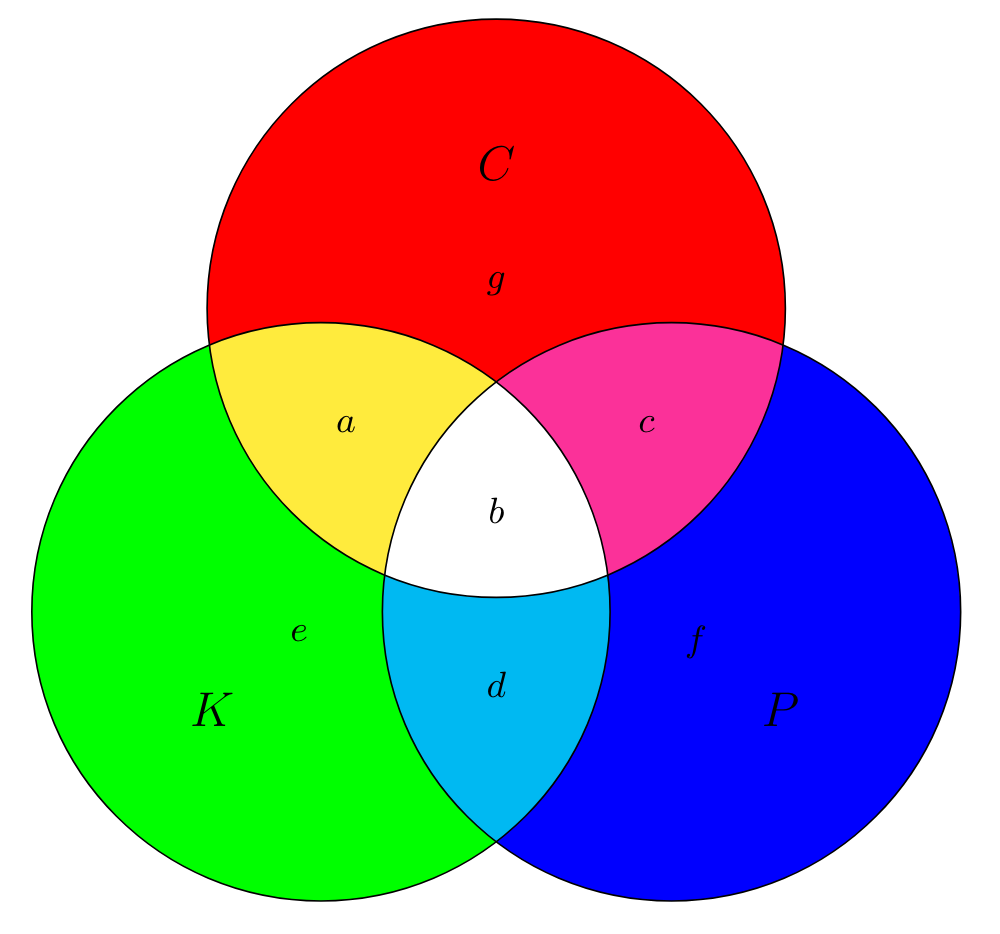
\includegraphics[width=0.5\textwidth]{entropy_diagram}
\end{figure}

\section*{Exercise 5.5}

By theorem 5.11 from the textbook, we that
$$
    H(K|C) = H(K) + H(P) - H(C)
$$

Since we are encyrpting one letter using the affine cipher,
the plaintext space is the same as
the ciphertext space, i.e. the alphabat, and the enrcyption
function is a bijection, we know that the plaintext
and the ciphertext has the same distribution and hence
$H(P) = H(C)$.

In the affine cipher, the coefficient $a$ must be invertible
with respect the modulo 26, leaving us 12 chioces for $a$,
which we denote as set $A$.
Therefore,
$$H(K|C) = H(K) = \sum_{K=(a,b)}^{A \times B}  Pr[K=(a,b)] \log \frac{1}{Pr[K=(a,b)]}$$

Because the choice of the key is uniformly random, we have
$$H(K|C) = \log 312$$ where $312$ comes from $12*26$.

\begin{equation*}
    \begin{split}
        & H(K|P,C) \\
        & = \sum_{i=0}^{25} \sum_{j=0}^{25} Pr[P=i, C=j] \cdot H(K|P=i,C=j) \\
        & = \sum_{i=0}^{25} \sum_{j=0}^{25} Pr[P=i, C=j] \cdot \left( \sum_{K=(a,b)}^{A \times B} Pr[K=(a,b)|P=i,C=j] \cdot \log \frac{1}{Pr[K=(a,b)|P=i,C=j]} \right)
    \end{split}
\end{equation*}

Because given the plaintext and the ciphertext, there are 12 equally
probable choices for $a$, and when $a$ is fixed, $b$ is fixed,
we then have

\begin{equation*}
    \begin{split}
        & Pr[K=(a,b)|P=i,C=j] \cdot \log \frac{1}{Pr[K=(a,b)|P=i,C=j]}  \\
        & =
        \begin{cases}
            \frac{1}{12} \log 12 & \text{if } a \cdot i + b \equiv j \text{ (and there are 12 such pairs of a and b)} \\
            0                    & \text{otherwise}
        \end{cases}
    \end{split}
\end{equation*}


Therefore,

$$
    H(K|P,C) = \sum_{i=0}^{25} \sum_{j=0}^{25} Pr[P=i, C=j] \cdot \log 12 = \log 12
$$

Intuitively, the results mean that when using the affine cipher
to encrypt one letter with uniformly random key $a$ and $b$,
the uncertainty of the key after seeing the ciphertext is
not changed, and the uncertainty of the key after seeing both
the plaintext and the ciphertext is the uncertainty of the
choice of $a$.

\end{document}
